\documentclass[letterpaper, 11pt]{extarticle}
\usepackage{ifxetex}
\ifxetex
    \usepackage{fontspec}
    \defaultfontfeatures{Ligatures={TeX}}
    \setmainfont{Arial}
\else % pdflatex
    \usepackage{lmodern}            
    \renewcommand{\familydefault}{\sfdefault}
    \usepackage[T1]{fontenc}       
    \usepackage[utf8]{inputenc}
\fi


\usepackage[nolist]{acronym}
\usepackage{booktabs}

% ==================================================
\usepackage{tikz}
\usetikzlibrary{patterns}
\usetikzlibrary{calc}
\usetikzlibrary{shapes, arrows, positioning}

\tikzset{arrows={[scale=2.0]}}

\newcommand{\customSingleBox}[4]{%
  \node[
    draw,
    minimum width=1cm,
    minimum height=1cm,
    anchor=center,
    align=center,
    fill=#4!50
  ] (#1) at (#2) {#3};
}

\newcommand{\customMiniBox}[4]{%
  \node[
    draw,
    minimum width=0.5cm,
    minimum height=0.5cm,
    anchor=center,
    align=center,
    fill=#4!50
  ] (#1) at (#2) {#3};
}

\newcommand{\customDecBox}[3]{%
  \node[
    draw,
    diamond,
    minimum width=2cm,
    minimum height=1cm,
    inner sep=0cm,
    anchor=center,
    align=center,
    fill=orange!50
  ] (#1) at (#2) {#3};
}

\newcommand{\customTerminator}[4]{%
  \node[
    draw,
    shape=ellipse,
    minimum width=2cm,
    minimum height=1cm,
    anchor=center,
    align=center,
    fill=#4!50
  ] (#1) at (#2) {#3};
}

\newcommand{\customInputBox}[4]{%
  \node[
    draw,
    trapezium,
    trapezium left angle=70,
    trapezium right angle=110,
    minimum width=1cm,
    minimum height=1cm,
    anchor=center,
    align=center,
    fill=#4!50
  ] (#1) at (#2) {#3};
}

\newcommand{\customOutputBox}[4]{%
  \node[
    draw,
    shape=display,
    minimum width=3cm,
    minimum height=1.5cm,
    anchor=center,
    align=center,
    fill=#4!50
  ] (#1) at (#2) {#3};
}

\usepackage{pgfplots}
\pgfplotsset{compat=1.18}

\usepackage[separate-uncertainty = true,multi-part-units=single]{siunitx}
\DeclareSIUnit\rad{rad}
\DeclareSIUnit\radSi{rad(Si)}
\DeclareSIUnit\gy{Gy}
\DeclareSIUnit\protons{protons}
\DeclareSIUnit\ions{ions}
\DeclareSIUnit\ev{eV}
\DeclareSIUnit\mbar{mbar}
\DeclareSIUnit\bar{bar}
\DeclareSIUnit\oct{oct}
\DeclareSIUnit\gn{g_{n}}
\DeclareSIUnit\rms{RMS}
\DeclareSIUnit\vrms{V\subs{rms}}
\DeclareSIUnit\usd{\$}
\sisetup{detect-weight,detect-mode}
\sisetup{per-mode=fraction}
\sisetup{exponent-product=\cdot}

\usepackage{tikz-timing}
\usetikztiminglibrary[rising arrows]{clockarrows}
\NewDocumentCommand{\busref}{som}{\texttt{%
#3%
\IfValueTF{#2}{[#2]}{}%
\IfBooleanTF{#1}{\#}{}%
}}

% Miscellaneous packages
\usepackage{float}
\usepackage{tabularx}
\usepackage{xcolor}
\usepackage{multicol}
\usepackage{subcaption}
\usepackage{caption}
\captionsetup{format = hang, margin = 10pt, font = small, labelfont = bf}

% Packages for math
\usepackage{mathrsfs}
\usepackage{amsfonts}
\usepackage{amsmath}
\usepackage{amsthm}
\usepackage{amssymb}
\usepackage{physics}
\usepackage{dsfont}
\usepackage{esint}

\usepackage{colortbl}
   \definecolor{Gray}{gray}{0.85}
   \definecolor{LightCyan}{rgb}{0.88,1,1}
% ==================================================

% Packages for writing
\usepackage{enumerate}
\usepackage[shortlabels]{enumitem}
\usepackage{framed}
\usepackage{csquotes}

% Hyperlinks setup
\usepackage{hyperref}
\definecolor{links}{rgb}{0.36,0.54,0.66}
\hypersetup{
   colorlinks = true,
    linkcolor = black,
     urlcolor = blue,
    citecolor = blue,
    filecolor = blue,
    pdfauthor = {Author},
     pdftitle = {Title},
   pdfsubject = {subject},
  pdfkeywords = {one, two},
  pdfproducer = {LaTeX},
   pdfcreator = {pdfLaTeX},
   }

% Novo comando para definir entre inglês ou português
\newif\ifenglish\englishfalse
\englishtrue
\newcommand{\lang}[2]{\ifenglish#1\else#2\fi}

% ==================================================

% document parameters
% \usepackage[spanish, mexico, es-lcroman]{babel}
\englishfalse
\lang{
\usepackage[english]{babel}
\usepackage[margin = 1in]{geometry}}
{\usepackage[portuguese]{babel}
\usepackage[margin = 1in]{geometry}}

\newcommand{\DAY}{\the\day}
\newcommand{\MONTH}{%
    \ifcase\month
    \or \lang{January}{janeiro}%
    \or \lang{February}{fevereiro}%
    \or \lang{March}{março}%
    \or \lang{April}{abril}%
    \or \lang{May}{maio}%
    \or \lang{June}{junho}%
    \or \lang{July}{julho}%
    \or \lang{August}{agosto}%
    \or \lang{September}{setembro}%
    \or \lang{October}{outubro}%
    \or \lang{November}{novembro}%
    \or \lang{December}{dezembro}%
    \fi}
\newcommand{\YEAR}{\the\year}

\usepackage{titlesec}
\usepackage{listings}
\usepackage[most, minted]{tcolorbox}
%\usemintedstyle{vs}
%\usemintedstyle{pastie}
%\usemintedstyle{autumn}
%\usemintedstyle{emacs}
\usemintedstyle{bw}
%\usemintedstyle{colorful}

\renewcommand{\theFancyVerbLine}{\textcolor{black}{\scriptsize\arabic{FancyVerbLine}}}

\newtcblisting{mylisting}[4][]{
  arc=0pt, outer arc=0pt,
  listing only, 
  minted options app={#4},
  minted language=#3,
  title=#2,
  breakable,
  bottomsep at break=14.8pt,
  topsep at break=14.8pt,
  #1
}

% Adjust spacing after the chapter title
\titlespacing*{\chapter}{0cm}{-2.0cm}{0.50cm}
\titlespacing*{\section}{0cm}{0.50cm}{0.25cm}

% Indent 
\setlength{\parindent}{0pt}
\setlength{\parskip}{1ex}

% --- Theorems, lemma, corollary, postulate, definition ---
% \numberwithin{equation}{section}

\newtcbtheorem[]{problem}{Exercício}%
    {enhanced,
    colback = black!5, %white,
    colbacktitle = black!5,
    coltitle = black,
    boxrule = 0pt,
    frame hidden,
    borderline west = {0.5mm}{0.0mm}{black},
    fonttitle = \bfseries\sffamily,
    breakable,
    before skip = 3ex,
    after skip = 3ex
}{problem}

\tcbuselibrary{skins, breakable}

% --- You can define your own color box. Just copy the previous \newtcbtheorm definition and use the colors of yout liking and the title you want to use.

% --- Basic commands ---
%   Euler's constant
\newcommand{\eu}{\mathrm{e}}

%   Imaginary unit
\newcommand{\im}{\mathrm{i}}

%   Sexagesimal degree symbol
\newcommand{\grado}{\,^{\circ}}

% --- Comandos para álgebra lineal ---
% Matrix transpose
\newcommand{\transpose}[1]{{#1}^{\mathsf{T}}}

%%% Comandos para cálculo
%   Definite integral from -\infty to +\infty
\newcommand{\Int}{\int\limits_{-\infty}^{\infty}}

%   Indefinite integral
\newcommand{\rint}[2]{\int{#1}\dd{#2}}

%  Definite integral
\newcommand{\Rint}[4]{\int\limits_{#1}^{#2}{#3}\dd{#4}}

%   Dot product symbol (use the command \bigcdot)
\makeatletter
\newcommand*\bigcdot{\mathpalette\bigcdot@{.5}}
\newcommand*\bigcdot@[2]{\mathbin{\vcenter{\hbox{\scalebox{#2}{$\m@th#1\bullet$}}}}}
\makeatother

%   Hamiltonian
\newcommand{\Ham}{\hat{\mathcal{H}}}

%   Trace
\renewcommand{\Tr}{\mathrm{Tr}}

% Christoffel symbol of the second kind
\newcommand{\christoffelsecond}[4]{\dfrac{1}{2}g^{#3 #4}(\partial_{#1} g_{#2 #4} + \partial_{#2} g_{#1 #4} - \partial_{#4} g_{#1 #2})}

% Riemann curvature tensor
\newcommand{\riemanncurvature}[5]{\partial_{#3} \Gamma_{#4 #2}^{#1} - \partial_{#4} \Gamma_{#3 #2}^{#1} + \Gamma_{#3 #5}^{#1} \Gamma_{#4 #2}^{#5} - \Gamma_{#4 #5}^{#1} \Gamma_{#3 #2}^{#5}}

% Covariant Riemann curvature tensor
\newcommand{\covariantriemanncurvature}[5]{g_{#1 #5} R^{#5}{}_{#2 #3 #4}}

% Ricci tensor
\newcommand{\riccitensor}[5]{g_{#1 #5} R^{#5}{}_{#2 #3 #4}}

% https://tex.stackexchange.com/questions/428163/display-shape-for-flowchart-with-tikz
\makeatletter

\pgfdeclareshape{display}
{
  \inheritsavedanchors[from=rectangle] % this is nearly a rectangle
  \inheritanchorborder[from=rectangle]
  \inheritanchor[from=rectangle]{north}
  \inheritanchor[from=rectangle]{west}
  \inheritanchor[from=rectangle]{east}
  \inheritanchor[from=rectangle]{south}
  \inheritanchor[from=rectangle]{center}
  \inheritbackgroundpath[from=rectangle]
  \backgroundpath{
    % points
    \southwest \pgf@xa=\pgf@x \pgf@ya=\pgf@y
    \northeast \pgf@xb=\pgf@x \pgf@yb=\pgf@y
    % dimensions
    \pgfmathsetlength{\pgfutil@tempdima}{\pgf@xb-\pgf@xa}
    \pgfmathsetlength{\pgfutil@tempdimb}{\pgf@yb-\pgf@ya}
    % path
    \pgfpathmoveto{\pgfpointadd{\pgfqpoint{\pgf@xa}{\pgf@ya}}{\pgfqpoint{0.2\pgfutil@tempdima}{0pt}}}
    \pgfpathlineto{\pgfpointadd{\pgfqpoint{\pgf@xa}{\pgf@ya}}{\pgfqpoint{0pt}{0.5\pgfutil@tempdimb}}}
    \pgfpathlineto{\pgfpointadd{\pgfqpoint{\pgf@xa}{\pgf@yb}}{\pgfqpoint{0.2\pgfutil@tempdima}{0pt}}}    
    \pgfpathlineto{\pgfpointadd{\pgfqpoint{\pgf@xb}{\pgf@yb}}{\pgfqpoint{-0.2\pgfutil@tempdima}{0pt}}}
    \pgfpatharc{90}{-90}{0.2\pgfutil@tempdima and 0.5\pgfutil@tempdimb}
    \pgfpathlineto{\pgfpointadd{\pgfqpoint{\pgf@xb}{\pgf@ya}}{\pgfqpoint{-0.2\pgfutil@tempdima}{0pt}}}
    \pgfpathlineto{\pgfpointadd{\pgfqpoint{\pgf@xa}{\pgf@ya}}{\pgfqpoint{0.2\pgfutil@tempdima}{0pt}}}
    \pgfpathclose    
  }
}


\makeatother

\newcommand{\pontos}[1]{\textbf{(#1 pts.)}:~}

\newenvironment{questao}[2][]{%
    \noindent\textbf{#2} \textbf{#1}%
    \ignorespaces
}{%
    \vspace{0.5cm}%
}


\begin{document}

\begin{Large}
    \textbf{PRG22105 --- Programação de Computadores II}
    
    Projeto \hfill \lang{blabla}{\DAY~de \MONTH~de \YEAR}
\end{Large}

\vspace{1ex}
\textbf{\lang{Lecturer:}{Professor:}} \text{João Cláudio Elsen Barcellos}, \href{mailto:joao.barcellos@ifsc.edu.br}{\texttt{joao.barcellos@ifsc.edu.br}}\\
\textbf{\lang{Student:}{Estudante:}}


\vspace{2ex}
\begin{problem}{Controlador para produção de cerveja artesanal}{interpretacao}

\textbf{Objetivo e visão geral:} Este projeto propõe o desenvolvimento de um sistema embarcado para auxiliar no processo de produção de cerveja artesanal. O sistema deve controlar, em tempo real, a temperatura do processo e acionar a agitação do mosto por meio de um mixer, conforme condições específicas. Para isso, devem ser empregadas técnicas de controle como PID ou ON/OFF com histerese. As decisões de controle devem se basear em curvas programáveis (temperatura versus tempo), que podem ser definidas pelo usuário ou pré-configuradas no sistema.\\ 

A lógica de controle pode ser implementada a partir de uma máquina de estados gerada automaticamente com a ferramenta Yakindu (atualmente chamada itemis CREATE), ou construída manualmente pelo aluno. Nos casos em que Yakindu for utilizado, espera-se que os métodos da interface gerada sejam corretamente implementados no código-fonte. Caso o aluno opte por construir a máquina de estados do zero, o sistema deverá ser estruturado usando conceitos de orientação a objetos em C++, com destaque para o uso de métodos virtuais e polimorfismo. Nessa abordagem, o sistema deve permitir uma versão embarcada (ESP32) e outra versão simulável no PC, com troca de implementações via herança ou composição polimórfica. O sistema, como um todo, é apresentado de forma sucinta na \autoref{fig:diagrama-cerveja}.\\

\vspace{1ex}
\textbf{Requisitos mínimos:}
\begin{enumerate}
    \item \textbf{Plataforma de controle:}
    \begin{itemize}
        \item Microcontrolador de 32 bits com suporte a I\textsuperscript{2}C, SPI e UART.
        \item Capacidade de operação em tempo real (bare-metal ou com RTOS).
    \end{itemize}

    \item \textbf{Sensores e atuações:}
    \begin{itemize}
        \item Leitura de temperatura via I\textsuperscript{2}C.
        \item Controle de resistências (heaters) via GPIO ou PWM.
        \item Controle de mixer via GPIO ou PWM.
    \end{itemize}

    \item \textbf{Controle:}
    \begin{itemize}
        \item Implementação de controle PID e/ou ON/OFF com histerese.
        \item Mixer deve ser ativado quando a diferença entre dois sensores de temperatura exceder \SI{1}{\degreeCelsius}.
    \end{itemize}

        \item \textbf{Máquina de estados:}
    \begin{itemize}
        \item A máquina de estados pode ser gerada com o Yakindu/itemis CREATE, com implementação dos métodos obrigatórios da interface.
        \item Alternativamente, o controle pode ser implementado manualmente em C++, desde que use métodos virtuais, polimorfismo e permita a simulação no PC.
        \item A versão simulada deve permitir que a lógica de decisão seja testada sem o hardware, via entradas simuladas e saídas controladas por abstrações.
    \end{itemize}

    \item \textbf{Curvas programáveis:}
    \begin{itemize}
        \item O sistema deve possuir uma curva padrão.
        \item Novas curvas podem ser inseridas via comunicação serial.
        \item As curvas devem descrever um perfil de temperatura em função do tempo.
    \end{itemize}

    \item \textbf{Interfaces:}
    \begin{itemize}
        \item Interfaces lógicas: GPIO, PWM, I\textsuperscript{2}C, UART.
        \item Comunicação com o PC via UART.
    \end{itemize}

    \item \textbf{Detecção de erros:}
    \begin{itemize}
        \item O sistema deve identificar falhas como ausência de leitura dos sensores.
        \item Deve alertar o usuário e desativar os atuadores para segurança.
    \end{itemize}

    \item \textbf{Documentação e repositório:}
    \begin{itemize}
        \item Projeto deve estar versionado em repositório GitHub.
        \item Recomenda-se uso de \texttt{Doxygen} para documentação do código.
    \end{itemize}

    \item \textbf{Funcionalidade adicional:}
    \begin{itemize}
        \item O estudante deve propor e implementar uma funcionalidade extra, como: alarme sonoro, registro de logs, visualização gráfica, modo de calibração, entre outros.
    \end{itemize}
\end{enumerate}

\vspace{1ex}
\textbf{Sugestão de entregas parciais:}
\begin{description}
    \item[Entrega 1:] Levantamento de requisitos, definição das curvas, modelagem da máquina de estados (manual ou Yakindu) e diagramas de sistema.
    \item[Entrega 2:] Implementação dos drivers de sensores e atuadores, controle básico (PID ou ON/OFF), e comunicação com o PC.
    \item[Entrega 3:] Integração final com mixer funcional, detecção de falhas, funcionalidade adicional, documentação completa e demonstração.
\end{description}

\vspace{1ex}
\textbf{Critérios de avaliação:}
\begin{itemize}
    \item Funcionamento dos módulos implementados
    \item Clareza e organização do código
    \item Uso de boas práticas de programação embarcada
    \item Qualidade da documentação
    \item Utilização efetiva do GitHub para controle de versão
\end{itemize}

\vspace{1ex}
\textbf{Observações:}
\begin{itemize}
    \item A implementação pode ser feita em C ou C++ (preferencialmente, C++).
    \item O sistema deve ser portável e preparado para execução em plataforma embarcada real (ESP32 ou equivalente).
    \item É permitida a simulação parcial de dispositivos, desde que devidamente descrita e justificada.
    \item A lógica de controle deve ser validável tanto em ambiente embarcado quanto em simulação no PC.
\end{itemize}

\begin{figure}[H]
\centering
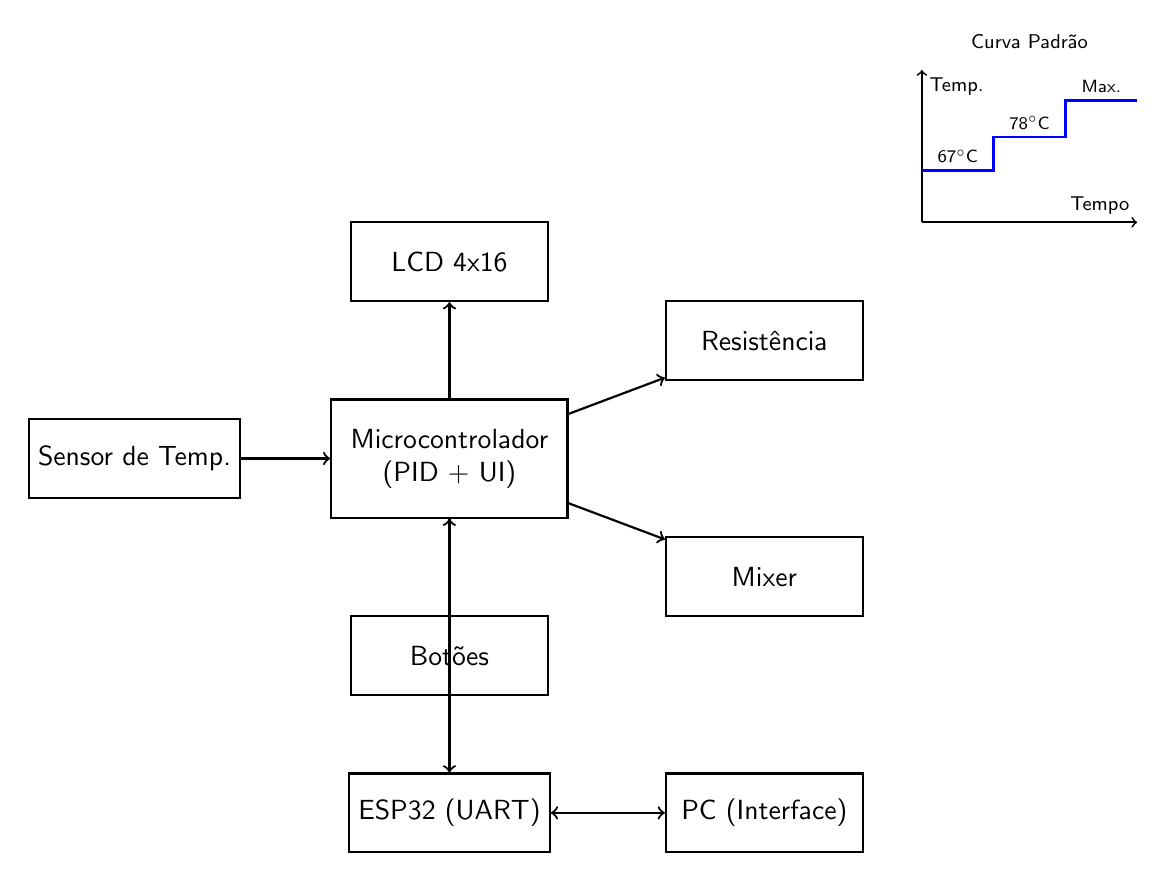
\begin{tikzpicture}[thick]

% --- Blocos principais ---
\node[draw, rectangle, minimum width=2.5cm, minimum height=1cm] (sensor) at (0,0) {Sensor de Temp.};
\node[draw, rectangle, minimum width=3cm, minimum height=1.5cm, align=center] (uC) at (4,0) {Microcontrolador\\(PID + UI)};
\node[draw, rectangle, minimum width=2.5cm, minimum height=1cm] (res) at (8,1.5) {Resistência};
\node[draw, rectangle, minimum width=2.5cm, minimum height=1cm] (mixer) at (8,-1.5) {Mixer};
\node[draw, rectangle, minimum width=2.5cm, minimum height=1cm] (lcd) at (4,2.5) {LCD 4x16};
\node[draw, rectangle, minimum width=2.5cm, minimum height=1cm] (btn) at (4,-2.5) {Botões};
\node[draw, rectangle, minimum width=2.5cm, minimum height=1cm] (esp) at (4,-4.5) {ESP32 (UART)};
\node[draw, rectangle, minimum width=2.5cm, minimum height=1cm] (pc) at (8,-4.5) {PC (Interface)};

% --- Setas ---
\draw[->] (sensor) -- (uC);
\draw[->] (uC) -- (res);
\draw[->] (uC) -- (mixer);
\draw[->] (uC) -- (lcd);
\draw[->] (btn) -- (uC);
\draw[<->] (esp) -- (pc);
\draw[->] (uC) -- (esp);

% --- Curva de temperatura padrão no canto superior direito ---
\begin{scope}[xshift=10cm, yshift=3cm, scale=0.8]
\begin{axis}[
    width=5cm,
    height=4cm,
    xmin=0, xmax=9,
    ymin=50, ymax=100,
    axis lines=middle,
    axis line style={->, thick},
    tick style={draw=none},
    xtick=\empty, ytick=\empty,
    xlabel={\small Tempo},
    ylabel={\small Temp.},
    title={Curva Padrão},
    title style={font=\small}
]

% Curva com três platôs
\addplot[very thick, blue, mark=none] coordinates {
    (0,67) (3,67)
    (3,78) (6,78)
    (6,90) (9,90)
};

% Anotações acima dos degraus
\node[anchor=south] at (axis cs:1.5,67) {\footnotesize 67\( ^\circ \)C};
\node[anchor=south] at (axis cs:4.5,78) {\footnotesize 78\( ^\circ \)C};
\node[anchor=south] at (axis cs:7.5,90) {\footnotesize Max.};

\end{axis}
\end{scope}



\end{tikzpicture}
\caption{\textcolor{red}{FIXME:} Diagrama geral do sistema de controle com curva padrão de temperatura.}
\label{fig:diagrama-cerveja}
\end{figure}


    
\end{problem}
    
\newpage

\vfill
\printbibliography

\end{document}
